% Basic US Letter document format
% by C. G. Wilson 
% modified by Morgan Fine-Morris

\documentclass[11pt]{article}
\usepackage{amsfonts}
\usepackage[pdftex]{graphicx}
\usepackage[space]{grffile}
\usepackage{caption}
\usepackage{subcaption}
\usepackage{placeins}

% \usepackage{palatino}

%%formatting
\textwidth 6.85in
\textheight 8.75in

\pagestyle{headings}
%\markright{\today, header}

\newcommand{\tsscale}{0.45}


\begin{document}

%%formatting
\oddsidemargin -0.22in
\evensidemargin -0.22in
\topmargin 0.05in
\topskip 0.25in
\headheight 0.05in
\headsep 0.25in

\graphicspath{{"../Data and Analysis/long TB Yan/plots/"}{"../Data and Analysis/short TB Yan/plots/"}}
%{"../Data and Analysis/long TB Yan/plots/Comparative TS Yan/"}{"../Data and Analysis/long TB Yan/plots/Comparative TS TB/"}}
%\begin{center}
%\Large{\textbf{Results}}
%\end{center}


\FloatBarrier
\section{Results}
talk about time series - what features characterize each model?
-Compare models by comparing features of their time series: Burst Duration, Interburst Interval, etc. 
From these generally trend are clear: as
Simple visual comparison of a section of membrane potential time series reveals the general trends created
Yan model characterized by longer burst duration and more spiking along the leading edge of each burst.
Comparing time series Figures ~\ref{fig:ts18} and ~\ref{fig:ts42}, we see that at the low end of the tested $g_{NaP}$ range (1.8 nS)...and at the end of the range, when $g_{NaP}$ = 4.2 nS, we see ...



\begin{figure}[h]
	\centering
	\subcaptionbox{Yan Model \label{fig:tsYan42}}{\includegraphics[scale=\tsscale]{Comparative TS Yan/ts_gnaps1p8_eLall.pdf}}%
	\subcaptionbox{TB Model \label{fig:tsTb42}}{\includegraphics[scale=\tsscale]{Comparative TS TB/ts_gnaps1p8_eLall.pdf}}
	\caption{Time series generated from Yan and TB models at all values of $eL$ for $g_{NaP}$ = 1.8 nS.}
	\label{fig:ts18}
	\subcaptionbox{Yan Model \label{fig:tsYan42}}{\includegraphics[scale=\tsscale]{Comparative TS Yan/ts_gnaps4p2_eLall.pdf}}%
	\subcaptionbox{TB Model \label{fig:tsTb42}}{\includegraphics[scale=\tsscale]{Comparative TS TB/ts_gnaps4p2_eLall.pdf}}
	\caption{Time series generated from Yan and TB models at all values of $eL$ for $g_{NaP}$ = 4.2 nS.}
	\label{fig:ts42}
\end{figure}

\begin{figure}[h]
	\centering
	\includegraphics[scale=\tsscale]{Comparative TS Yan/ts_gnaps1p8_eLall.pdf}
	\includegraphics[scale=\tsscale]{Comparative TS TB/ts_gnaps1p8_eLall.pdf}
	%\caption{Time series generated from Yan and TB models at all values of $eL$ for $g_{NaP}$ = 1.8 nS.}
	%\label{fig:ts18}
	\includegraphics[scale=\tsscale]{Comparative TS Yan/ts_gnaps4p2_eLall.pdf}
	\includegraphics[scale=\tsscale]{Comparative TS TB/ts_gnaps4p2_eLall.pdf}
	%\caption{Time series generated from Yan and TB models at all values of $eL$ for $g_{NaP}$ = 4.2 nS.}
	\label{fig:ts42}
\end{figure}

\subsection{Total Cycle Time, Burst Duration, Interburst Interval}


-Interesting to note that while most of the measures vary considerably depending on the model and parameters used to generate the time series, Total Cycle exhibits little-to-no change ~ref{fig:hm txt}. The single exception, caused by bi-modal bursting behavior ~\ref{fig:tsTb42}, occurs in the TB model when $eL$=-60.0 mV and $g_{NaP}$=4.2 nS. 

Average total cycle time, the time from the start of one burst to the start of another, was very uniform between models for all parameter sets that exhibited bursting (Fig [~\ref{fig:hm_tct}]). The only point of significant difference was at $eL=-60 g_{nap} = 4.2$ where the value for the TB model was half that of the Yan model, due to the two modes of interburst interval present in for the TB model but not for the Yan model (Fig [~\ref{fig:ts_6042}]).

\begin{figure}
	\centering
	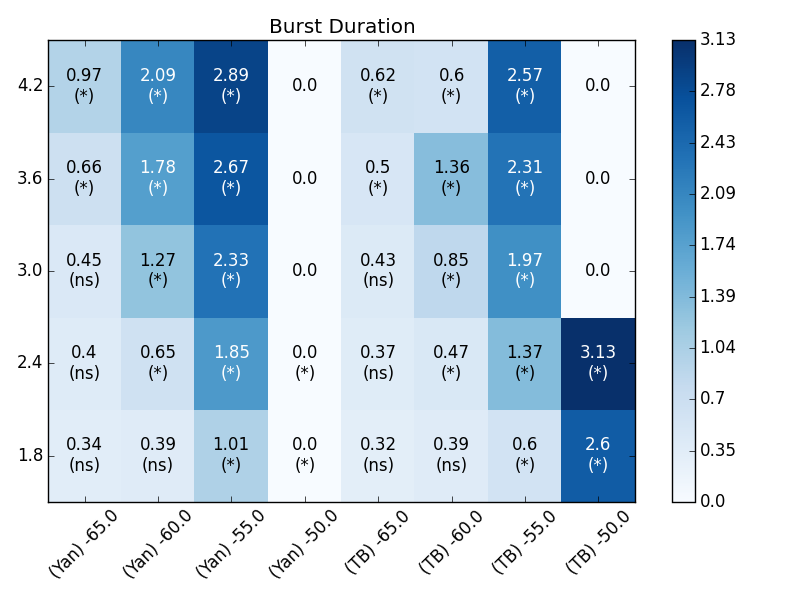
\includegraphics[scale=.4]{heatmap_Burst_Duration.png}
	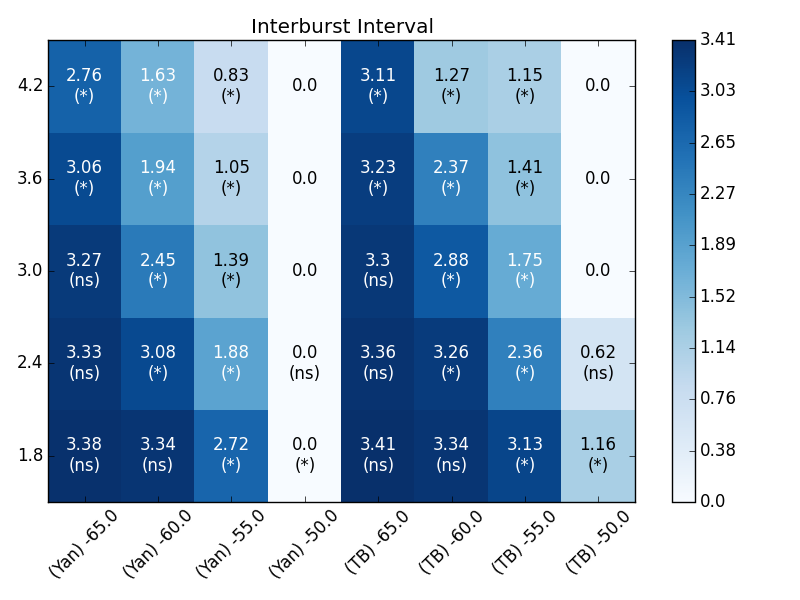
\includegraphics[scale=.4]{heatmap_Interburst_Interval.png}
	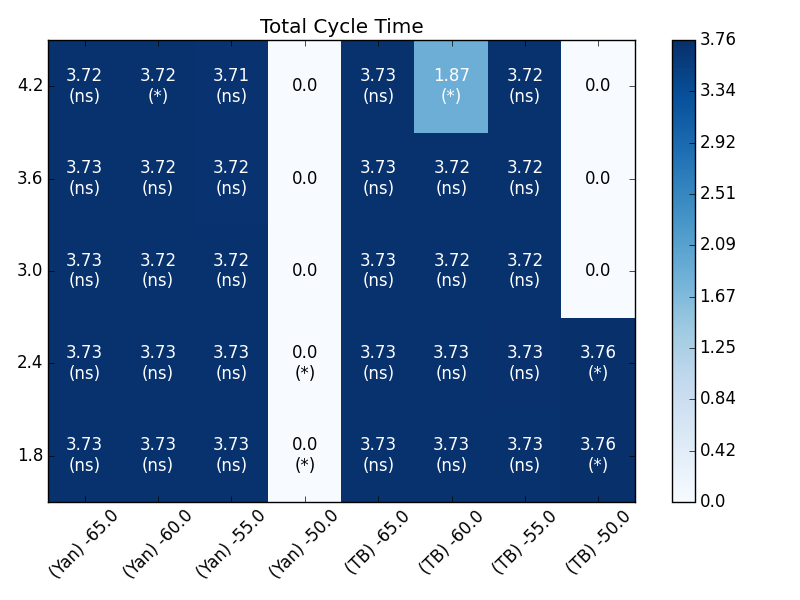
\includegraphics[scale=0.4]{heatmap_Total_Cycle_Time.png}
	\caption{Heat map showing variations in total cycle time with changes in $eL$, $g_{NaP}$, and model. Zeroes indicate tonic spiking.}
	\label{fig:hmTCT}
\end{figure}



\begin{figure}
	\centering
	\includegraphics[scale=0.4]{barchart_Burst_Duration.png}
\end{figure}

  \begin{figure}
	\centering
	\includegraphics[scale=0.4]{barchart_Interburst_Interval.png}
\end{figure} 
   


Where bursting occurs in the Yan model, burst duration for Yan increases more rapidly than TB as $eL$ increases. For $eL=-55 mV$, burst duration is different at all tested $g_{NaP}$ values.
Differences in burst duration between the two models does not change significantly with change in $g_{NaP}$. For Yan, bursting does not occur while $eL = -50 mV$, while bursting occurs at $eL=-50,\  g_{NaP}=1.8, 2.4$. 


While interburst interval and burst duration display the same pattern of significance, the patterns visible in their values are flipped. This is unsurprising, since Total Cycle Time, the summation of Interburst interval and burst duration, was nearly invariant across all model-parameter combinations. The only exception, for $eL=-50.0,\ g_{NaP} = 2.4$ where interburst interval for the TB model shrinks to 0.62 seconds, which is apparently not significantly different from 0.



\subsection{Peak within Bursts Measures}

\begin{figure}
\centering
	\subcaptionbox{Intraburst Frequency \label{fig:hmIF}}{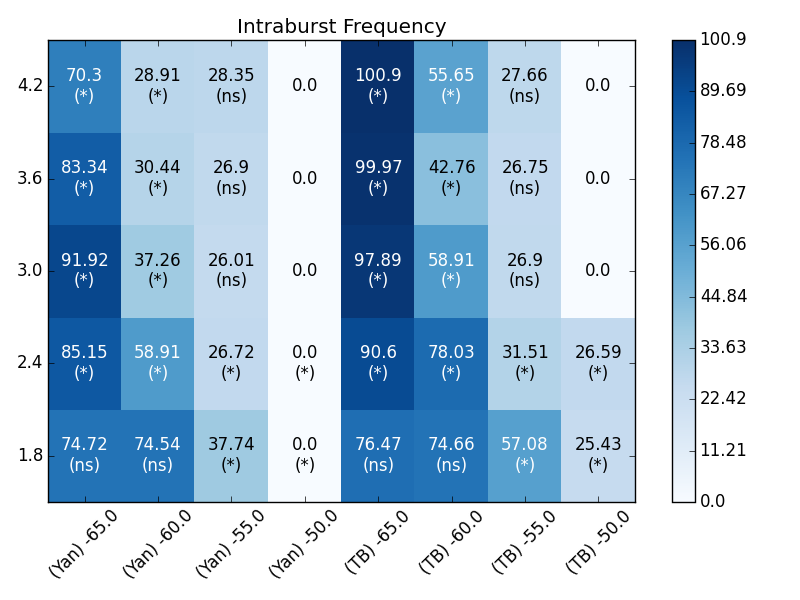
\includegraphics[scale=.4]{heatmap_Intraburst_Frequency.png}}%
	\subcaptionbox{Peaks per Burst \label{fig:hmPpB}}{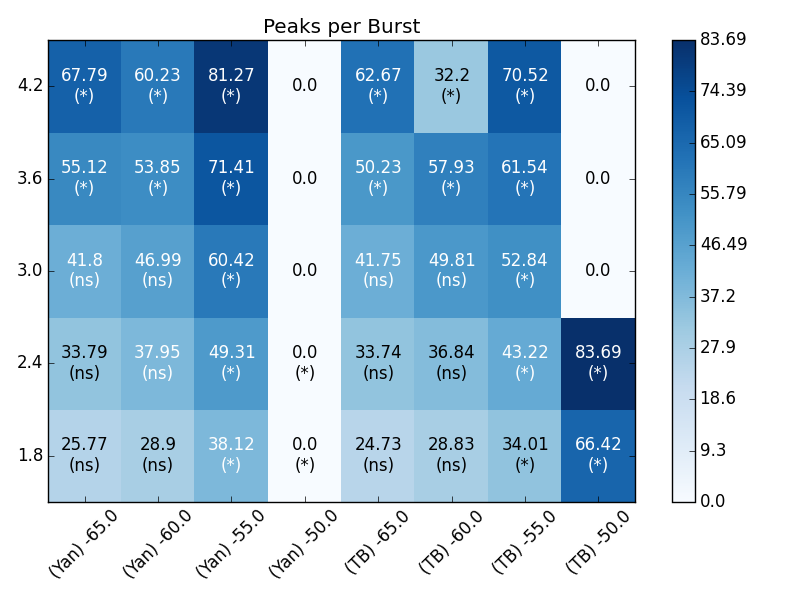
\includegraphics[scale=.4]{heatmap_Peaks_per_Burst.png}}%
	\caption{}
	\label{fig:hmPeakInBurst}
\end{figure}



\subsection{Peak Measures}
  
\begin{figure}
	\centering
	\subcaptionbox{Intraburst Frequency \label{fig:hmIF}}{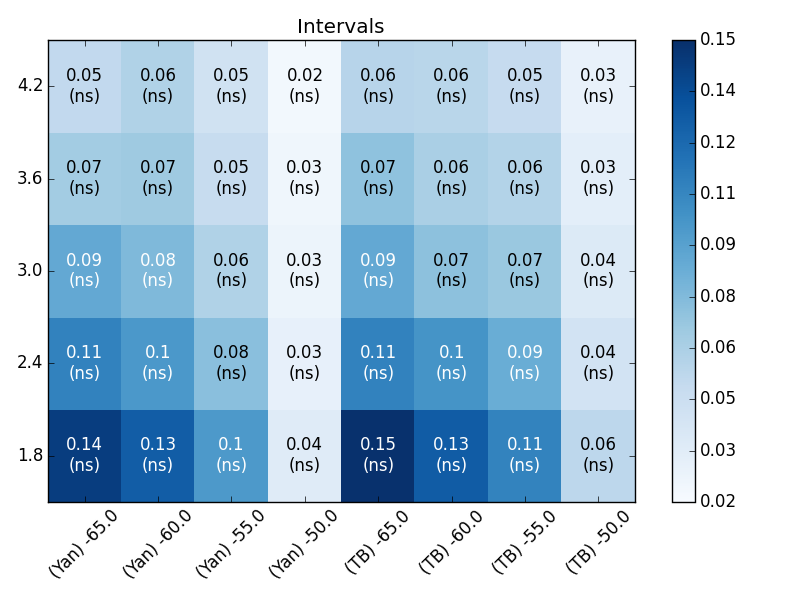
\includegraphics[scale=.4]{heatmap_Intervals.png}}%
	\subcaptionbox{Peaks per Burst \label{fig:hmPpB}}{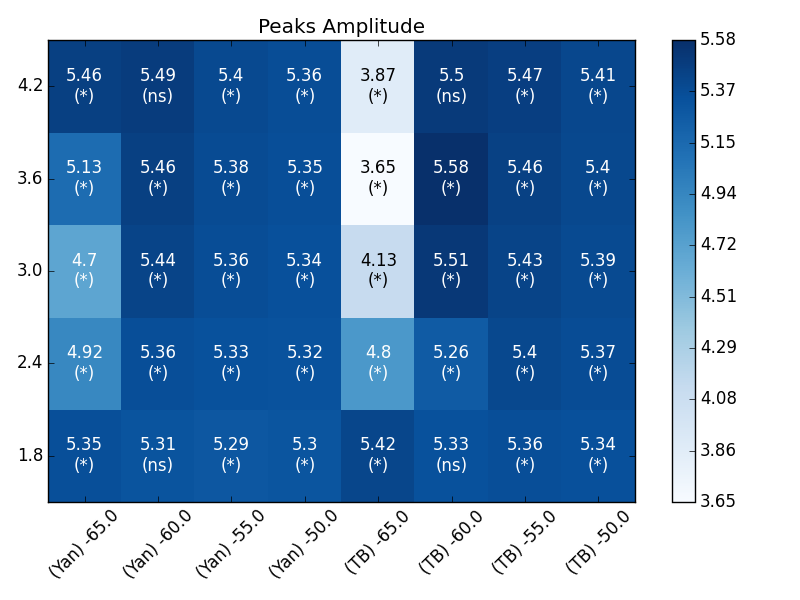
\includegraphics[scale=.4]{heatmap_Peaks_Amplitude.png}}%
	\caption{}
	\label{fig:hmPeaks}

\end{figure}
 

 
%\vspace{1.50cm}
%\noindent
\end{document}